%%%%%%%%%%%%%%%%%%%%%%%%%%%%%%%%%%%%%%%%%%%%%%%%%%%%%%%%%%%%%%%%%%%%%%%%%%%%%%%%%%%%%%%%%%%%%%%
%% Description:       Programmentwurf advanced software engineering
%% Author:      Manuel Berg, m.berg@enbw.com
%%  -*- coding: utf-8 -*-
%%%%%%%%%%%%%%%%%%%%%%%%%%%%%%%%%%%%%%%%%%%%%%%%%%%%%%%%%%%%%%%%%%%%%%%%%%%%%%%%%%%%%%%%%%%%%%%

\titlespacing*{\chapter}{0pt}{-30mm}{10pt}
\titleformat{\chapter}[display]
  {\normalfont\bfseries}{}{10pt}{\Huge\thechapter.\quad}
  
\chapter{Unit Tests (8P)}
\pagestyle{scrheadings}
\clearscrheadfoot
\pagenumbering{arabic}
\setcounter{page}{20}
\ofoot[\pagemark]{\pagemark}
%\ohead[\headmark]{\headmark}
\onehalfspacing

\section{10 Unit Tests (2P)}
\emph{[Nennung von 10 Unit-Tests und Beschreibung, was getestet wird]}

\begin{table}[htbp]
\centering
\centerline{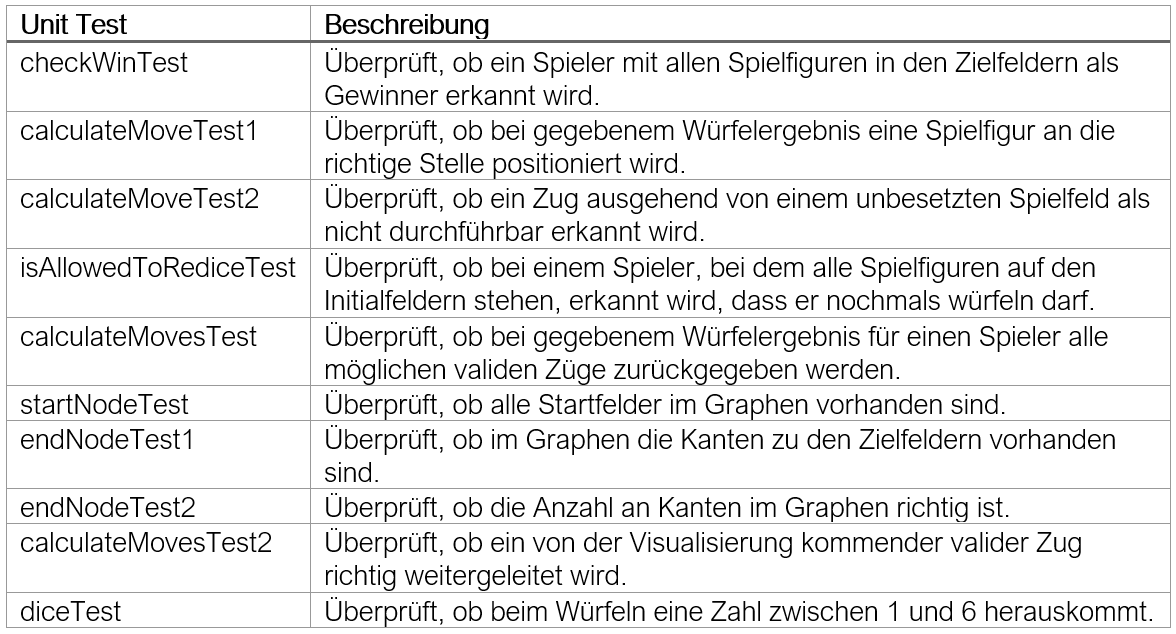
\includegraphics[scale=.55]{unitteststable}}
\caption{10 Unit Tests}
\label{tab:unitteststable}
\end{table}

\section{ATRIP: Automatic (1P)}
\emph{[Begründung/Erläuterung, wie ‘Automatic’ realisiert wurde]}
\vspace{.4cm}

\noindent Die Tests sind einfach auszuführen, denn es reicht auf dem Ordner, in dem alle Tests enthalten sind, das Starten aller Tests auszuwählen. Ein anderen Weg wäre das Ausführen des Befehls \textbf{\texttt{mvn clean test}}. Außerdem müssen bei keinem Test Daten manuell eingegeben werden. Somit laufen alle Tests automatisch ab. Des Weiteren überprüfen sich alle Tests selbst und geben als Ergebnis entweder bestanden oder fehlgeschlagen zurück.

\newpage
\section{ATRIP: Thorough (1P)}
\emph{[Code Coverage im Projekt analysieren und begründen]}
\vspace{.4cm}

\noindent Die Code Coverage im Projekt ist leider eher dürftig. Es wurden zwar die Kernfunktionen mit Tests abgedeckt, aber dennoch fehlen auch einige Aspekte, die wir als notwendig bezeichnen würden. Zum Beispiel gibt es keinerlei Tests zur GUI. Diese wurde nur händisch getestet.

Bei den Tests wurden einmal die möglichen Aktionen auf dem Spielbrett betrachtet. Hierzu zählen fünf ersten Tests aus der \hyperref[tab:unittesttable]{vorherigen Tabelle}. Außerdem wurde die dem Spielbrett zugrundeliegende Struktur, also der darunterliegende Graph, getestet. Hierbei sind aber auch nur cica 10\% des fertigen Graphen überprüft worden. Da dieser Graph zur Validierung von Zügen beisteuert ist dies eine kritische Stelle, die nicht mit Tests abgedeckt ist. Zum Schluss wurde dann noch der \enquote{GameService} mithilfe dreier Mocks getestet. Aber auch hier fehlt zum Beispiel die Überprüfung, ob ein neues Spiel richtig aufgebaut wird.

Bei der Erstellung der Tests wurde der Fokus auf die Kernfunktionalitäten gelegt. Es wurde aber beim Auftritt eines Fehlers dieser im Code verbessert und nicht direkt ein Test geschrieben. Zukünftig sollte das anders gehandhabt und auch direkt das Umfeld des Fehlers betrachtet werden.

\newpage
\section{ATRIP: Professional (1P)}
\emph{[jeweils 1 positves und negatives Beispiele zu ‘Professional’; jeweils Code-Beispiel, Analyse und
Begründung, was professionell/nicht professionell an den Beispielen ist]}

\begin{figure}[htbp]
\centering
\centerline{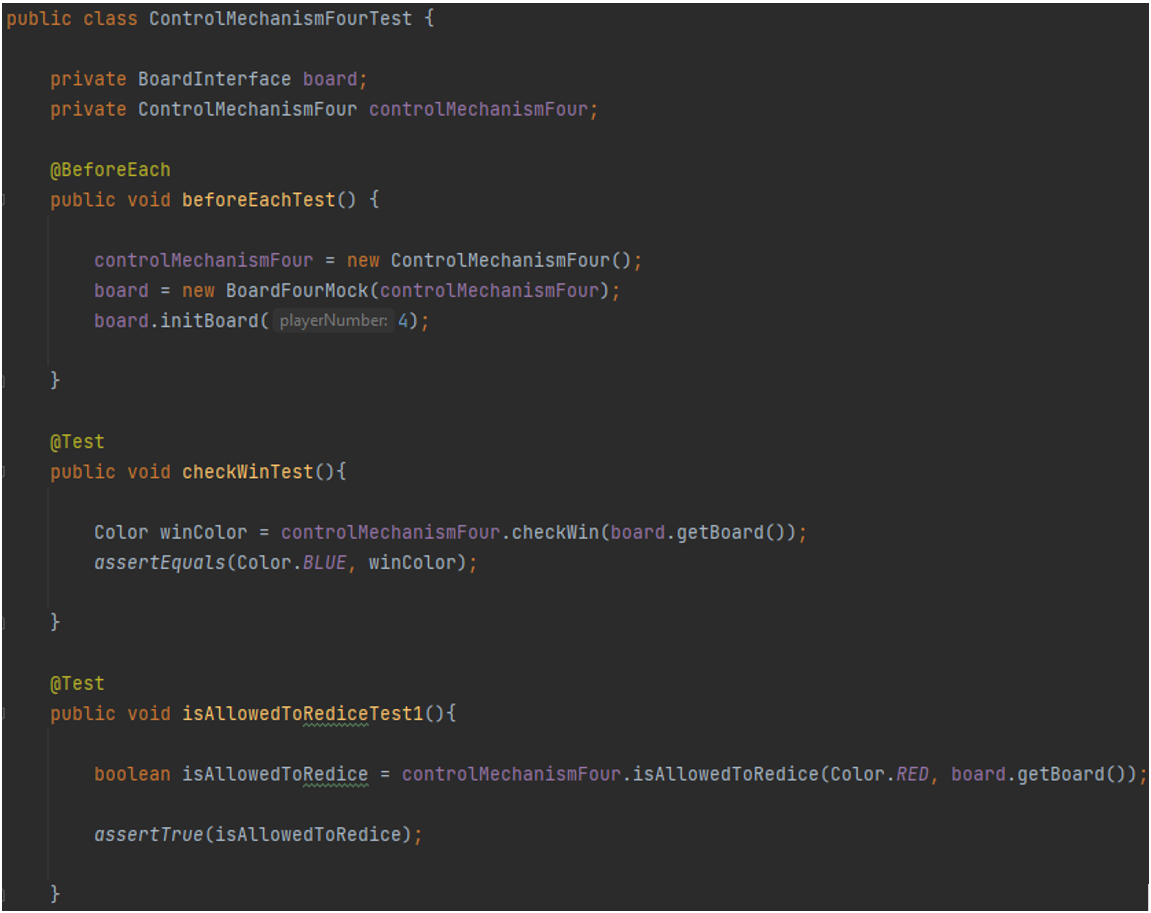
\includegraphics[scale=.5]{professional}}
\caption{Positiv-Beispiel Professional}
\label{fig:professional}
\end{figure}

\noindent Hier ist ein positives Beispiel zu \enquote{Professional} zu sehen. Es wird ein Mock für das Spielbrett eingesetzt. In der Testklasse werden verschiedene Aktionen beziehungsweise Funktionalitäten auf dem Spielbrett getestet. Hierbei wird der Code in der \enquote{beforeEachTest}-Methode wiederverwendet, was für \enquote{Professional} spricht. Hierdurch werden auch Fehlerquellen verkleinert, denn beispielsweise bei Änderungen muss hier nur eine Stelle im Code bedacht werden. Dies spricht auch für eine gute Code-Qualität.

\newpage

\begin{figure}[htbp]
\centering
\centerline{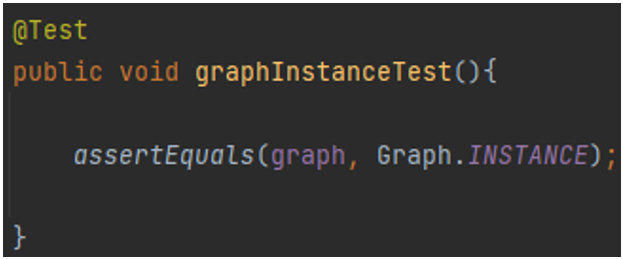
\includegraphics[scale=.5]{notprofessional}}
\caption{Negativ-Beispiel Professional}
\label{fig:notprofessional}
\end{figure}

\noindent Dieser Test überprüft, ob es tatsächlich nur eine Graph-Instanz gibt. Das ist aber sinnlos und ein Negativ-Beispiel zu \enquote{Professional}, da der Graph ein Singleton ist und somit nur eine Instanz existiert. 

\section{Fakes und Mocks (1P)}
\emph{[Analyse und Begründung des Einsatzes von 2 Fake/Mock-Objekten; zusätzlich jeweils UML
Diagramm der Klasse]}

\subsubsection{BoardFourMock}
\noindent Dieses Mock ist stellvertretend für ein Spielbrett. Dabei wurden nur die notwendigen Funktionalitäten implementiert. Das heißt, es gibt einen festen Spielstand der sozusagen \enquote{initialisiert} wird. Bei diesem Spielstand wurden absichtlich die Spielfiguren so gestellt, dass die möglichen Aktionen gut getestet werden können. Zum Beispiel ist die Farbe Blau im Ziel und somit kann die Funktion, ob jemand gewonnen hat, überprüft werden. Ein anderen Beispiel ist, dass Rot noch auf der Startposition steht und somit überprüft werden kann, ob Rot auch dreimal würfeln darf.

\begin{figure}[htbp]
\centering
\centerline{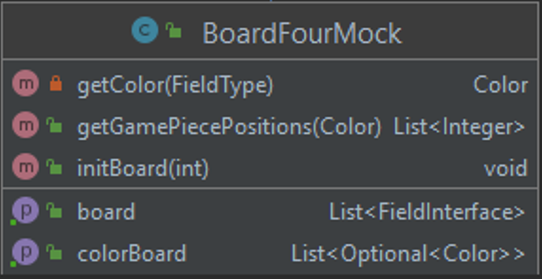
\includegraphics[scale=.5]{boardfourmock}}
\caption{BoardFourMock}
\label{fig:boardfourmock}
\end{figure}


\newpage
\subsubsection{GameFrameMock}
\noindent Das Mock \enquote{GameFrameMock} ist stellvertretend für die GUI da. Um den \enquote{GameService} ohne Abhängigkeiten testen zu können, wurden durch dieses Mock die minimal notwendigen Funktionalitäten geboten. Zum Beispiel konnte ohne die große GUI-Komponente mit einem akzeptablen Aufwand getestet werden, ob ein von der Visualisierung kommender valider Zug richtig weitergeleitet wird.

\begin{figure}[htbp]
\centering
\centerline{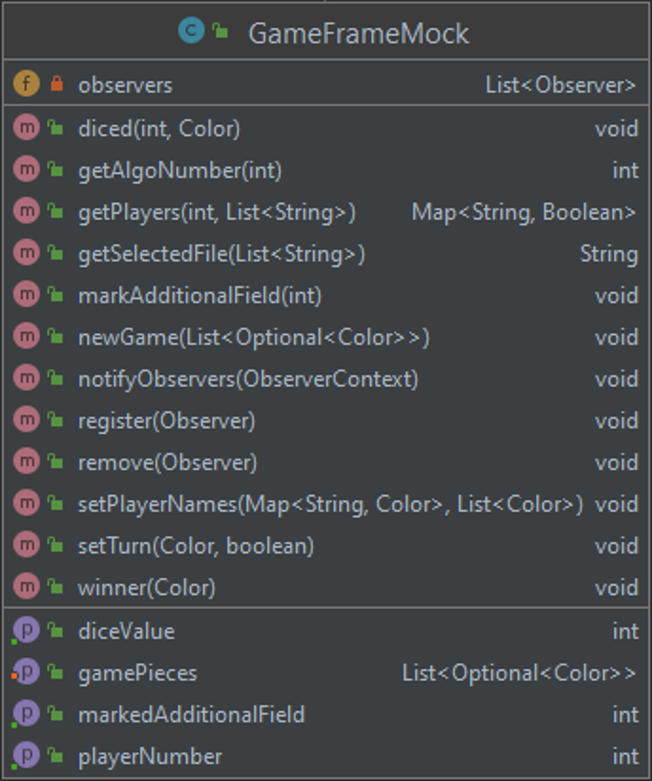
\includegraphics[scale=.5]{gameframemock}}
\caption{GameFrameMock}
\label{fig:gameframemock}
\end{figure}

\newpage
\titlespacing*{\chapter}{0pt}{-30mm}{10pt}
\titleformat{\chapter}[display]
  {\normalfont\bfseries}{}{10pt}{\Huge\thechapter.\quad}
  
\chapter{Domain Driven Design (8P)}
\pagestyle{scrheadings}
\clearscrheadfoot
\pagenumbering{arabic}
\setcounter{page}{25}
\ofoot[\pagemark]{\pagemark}
%\ohead[\headmark]{\headmark}
\onehalfspacing

\section{Ubiquitous Language (2P)}
\emph{[4 Beispiele für die Ubiquitous Language; jeweils Bezeichung, Bedeutung und kurze Begründung,
warum es zur Ubiquitous Language gehört]}

\begin{figure}[htbp]
\centering
\centerline{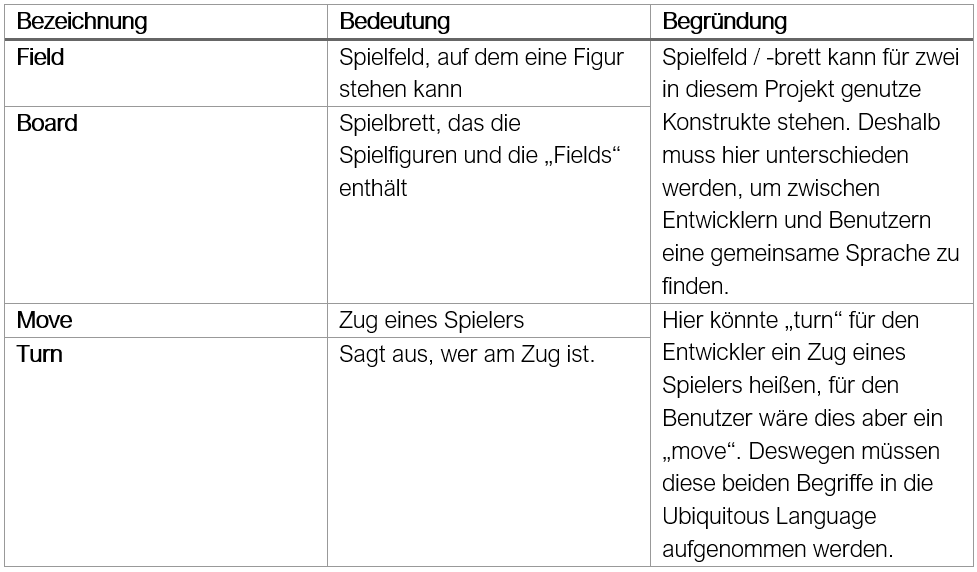
\includegraphics[scale=.7]{ubiquitous}}
\caption{4 Beispiele für die Ubiquitous Language}
\label{fig:ubiquitous}
\end{figure}

% \begin{table}[htbp]
% \centering
%     \begin{tabular}{|l|l|l|}
%         \hline
%         \textbf{Bezeichnung} & \textbf{Bedeutung} & \textbf{Begründung} \\ \hline
%         ~         & ~          & ~  \\ \hline
%         ~         & ~          & ~  \\ \hline
%         ~         & ~          & ~  \\ \hline
%         ~         & ~          & ~  \\ 

%         \hline
%     \end{tabular}
%     \label{Tab:ddd_examples}
%     \caption{4 Beispiele für die Ubiquitous Language}
% \end{table}

\section{Repositories (1,5P)}
\emph{[UML, Beschreibung und Begründung des Einsatzes eines Repositories; falls kein Repository
vorhanden: ausführliche Begründung, warum es keines geben kann/hier nicht sinnvoll ist]}

\noindent Das Repository wird durch die Klasse \enquote{GameIO} repräsentiert und bietet Zugriff auf persistenten Speicher. Außerdem wird die konkret verwendete Speichertechnologie vor dem Domain Code verborgen. In unserem Beispiel ist es das Abspeichern und Laden von Spielständen, was mithilfe von JSON umgesetzt wird. Dadurch kann ein Spiel unterbrochen und später fortgesetzt werden.

\section{Aggregates (1,5P)}
\emph{[UML, Beschreibung und Begründung des Einsatzes eines Aggregates; falls kein Aggregate
vorhanden: ausführliche Begründung, warum es keines geben kann/hier nicht sinnvoll ist]}

\begin{figure}[htbp]
\centering
\centerline{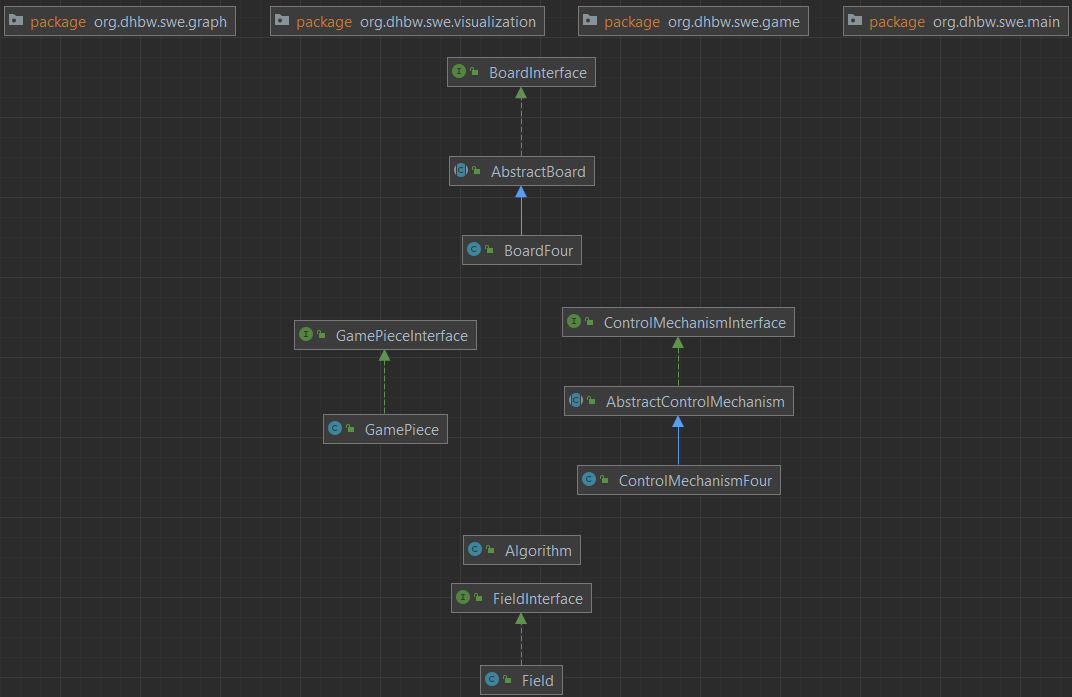
\includegraphics[scale=.6]{aggregat}}
\caption{Aggregate [Eigene Darstellung aus \emph{IntelliJ}]}
\label{fig:aggregat}
\end{figure}

\noindent Die in \hyperref[fig:aggregat]{Abbildung 6.2} dargestellten Klassen gehören zu einem Aggregat. Dies ist eine gemeinsam verwaltete Einheit und ist innerhalb seiner Grenzen konsistent. Durch diese Konsistenzgrenze war es sinnvoll, das Aggregat für das Spielbrett einzusetzen, da beispielsweise auch die Züge stets konsistent sein müssen. Als Aggregatswurzel fungiert das \enquote{BoardInterface}. Dieses kontrolliert alle Zugriffe auf das Aggregat. Wenn eines der vier oben dargestellten Packages Änderungen am Spielbrett vornehmen möchte, geht dies nur über die Aggregatswurzel. 

\section{Entities (1,5P)}
\emph{[UML, Beschreibung und Begründung des Einsatzes einer Entity; falls keine Entity vorhanden:
ausführliche Begründung, warum es keines geben kann/hier nicht sinnvoll ist]}

\begin{figure}[htbp]
\centering
\centerline{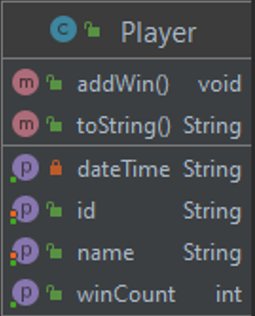
\includegraphics[scale=.6]{entities}}
\caption{Entitiy Player [Eigene Darstellung aus \emph{IntelliJ}]}
\label{fig:entities}
\end{figure}

\noindent Jeder Player hat eine eindeutige Identität. Alle Spieler, die jemals teilgenommen haben, werden in einer JSON-Datei gespeichert und durch die \enquote{id} identifiziert. Dadurch kann auch die insgesamte Anzahl an Gewinnen abgespeichert werden. Anhand dieser sich über die Zeit verändernden Zahl \enquote{} ist zu erkennen, dass der \enquote{Player} veränderliche Eigenschaften und einen Lebenszyklus hat. 

Aufgrund der Anforderungen waren hier eine Identität und veränderliche Eigenschaften notwendig. Da dies Merkmale einer Entity sind war es hier sinnvoll den \enquote{Player} als eine solche zu implementieren.

\newpage
\section{Value Objects (1,5P)}
\emph{[UML, Beschreibung und Begründung des Einsatzes eines Value Objects; falls kein Value Object
vorhanden: ausführliche Begründung, warum es keines geben kann/hier nicht sinnvoll ist]}

\begin{figure}[htbp]
\centering
\centerline{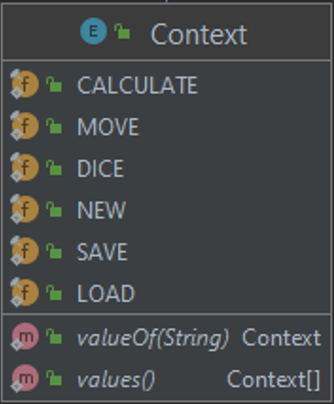
\includegraphics[scale=.6]{valueobjects}}
\caption{Enum als Value Object [Eigene Darstellung aus \emph{IntelliJ}]}
\label{fig:valueobjects}
\end{figure}

\noindent Ein Enum hat keine Identität, was auch auf Value Objects zutrifft. Außerdem sind Value Objects gleich, wenn sie denselben Wert haben. Dies lässt sich einfach durch \textbf{\texttt{Context.DICE.equals(Context.DICE)}}. Da dies wahr ist, trifft auch dieser Aspekt des ValueObject auf das \enquote{Context}-Enum zu. Des Weiteren haben ValueObjects keinen Lebenszyklkus, was auch hier passt. Da das \enquote{Context}-Enum keine Instanzvariablen besitzt ist es auch unveränderlich. Das bedeutet nicht alle Enums sind Value Objects, aber das hier gezeigte Enum ist eines.

% \begin{figure}[htbp]
% \centering
% \centerline{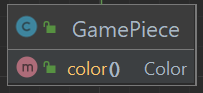
\includegraphics[scale=.6]{valueobject}}
% \caption{Value Object [Eigene Darstellung aus \emph{IntelliJ}]}
% \label{fig:valueobject}
% \end{figure}

% \noindent Ein Value Object ist hier eine Spielfigur. Diese hat als Eigenschaft nur die Farbe, welche über den gesamten Zeitraum hinweg unveränderlich bleibt. Die Änderung der Farbe ist nur durch die Konstruktion eines neuen Objektes möglich. Die Spielfigur besitzt keine eigene Identität und es ist auch kein Lebenszyklus erkennbar.

% Bezüglich des \enquote{GamePiece} sind das Überschreiben von \enquote{equals()} und \enquote{hashCode()} sowie die weiteren Vorgaben aus der Vorlesung zur Implementierung von Value Objects in Java beachtet worden.

\newpage
\titlespacing*{\chapter}{0pt}{-30mm}{10pt}
\titleformat{\chapter}[display]
  {\normalfont\bfseries}{}{10pt}{\Huge\thechapter.\quad}
  
\chapter{Refactoring (8P)}
\pagestyle{scrheadings}
\clearscrheadfoot
\pagenumbering{arabic}
\setcounter{page}{29}
\ofoot[\pagemark]{\pagemark}
%\ohead[\headmark]{\headmark}
\onehalfspacing

\section{Code Smells (2P)}
\emph{[jeweils 1 Code-Beispiel zu 2 unterschiedlichen Code Smells aus der Vorlesung; jeweils Code-Beispiel
und einen möglichen Lösungsweg bzw. den genommen Lösungsweg beschreiben (inkl. (Pseudo-)Code)]}

\subsubsection{Long Method}
\noindent Dieser Code Smell war in der \enquote{calculateTurn}-Methode in der \enquote{ControlMechanismFour}-Klasse enthalten. Wie in \hyperref[fig:longmethod]{Abbildung 7.1} ersichtlich, ist die Methode viel zu lang. Zusätzlich mussten noch Kommentare eingefügt werden, dass die Methode überhaupt einigermaßen verständlich ist. 

Nach der Eliminierung des Code Smells sind nur noch die drei logischen Möglichkeiten nach den Spielregeln in der Methode enthalten. Das eigentliche Berechnen der Züge ist ausgelagert. Durch die Methodennamen sind auch keine Kommentare mehr notwendig.

\begin{figure}[htbp]
\centering
\centerline{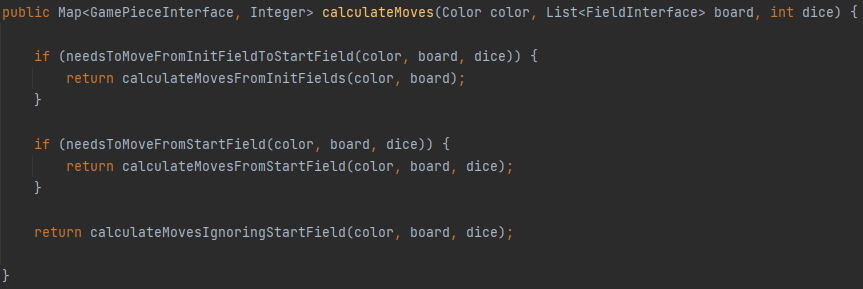
\includegraphics[scale=.5]{longmethodsolution}}
\caption{Eliminierung der Long Method [Eigene Darstellung aus \emph{IntelliJ}]}
\label{fig:longmethodsolution}
\end{figure}

\begin{figure}[htbp]
\centering
\centerline{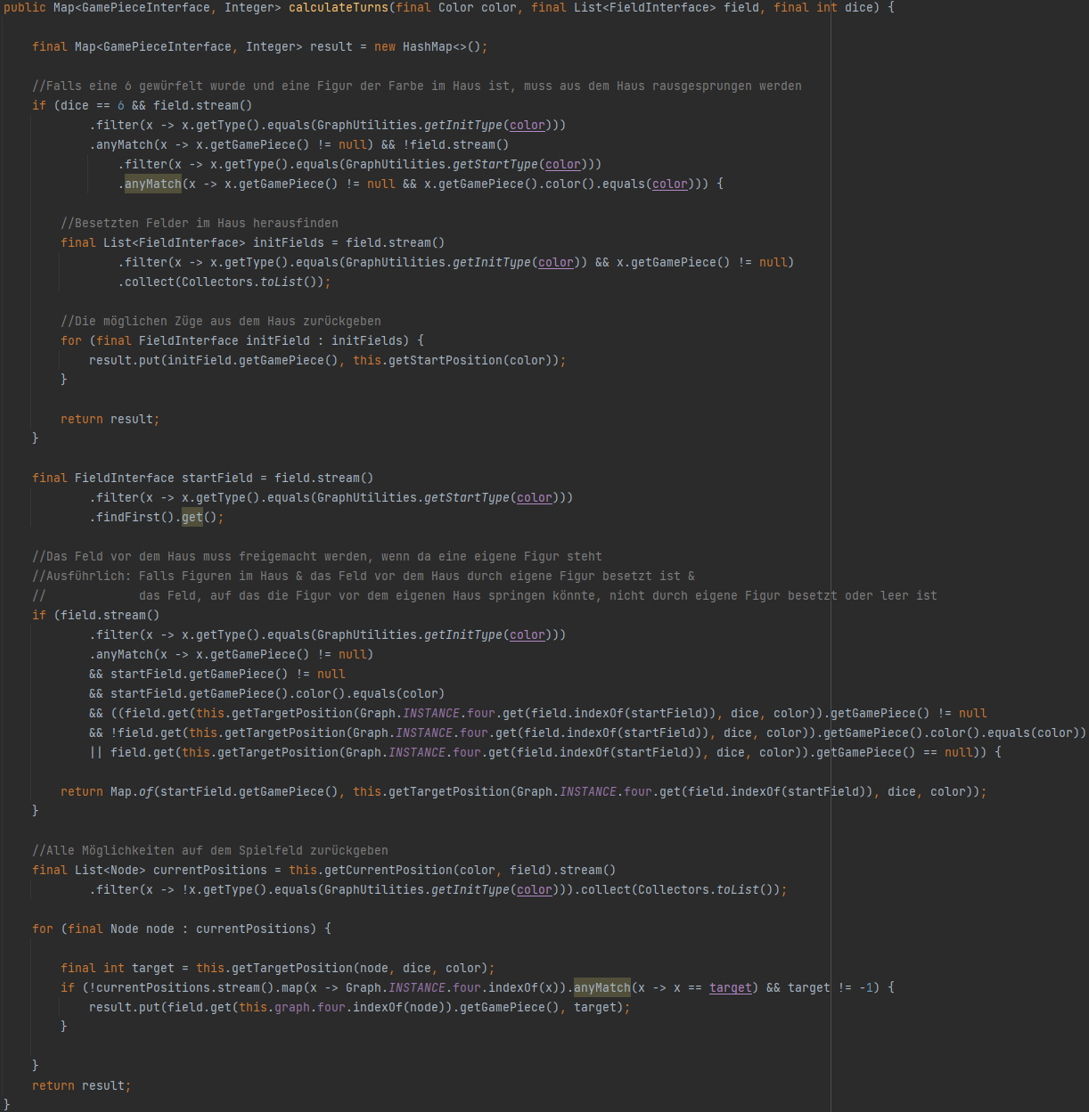
\includegraphics[scale=.65]{longmethod}}
\caption{Long Method [Eigene Darstellung aus \emph{IntelliJ}]}
\label{fig:longmethod}
\end{figure}

\newpage

\subsubsection{Switch-Statements}

\begin{figure}[htbp]
\centering
\centerline{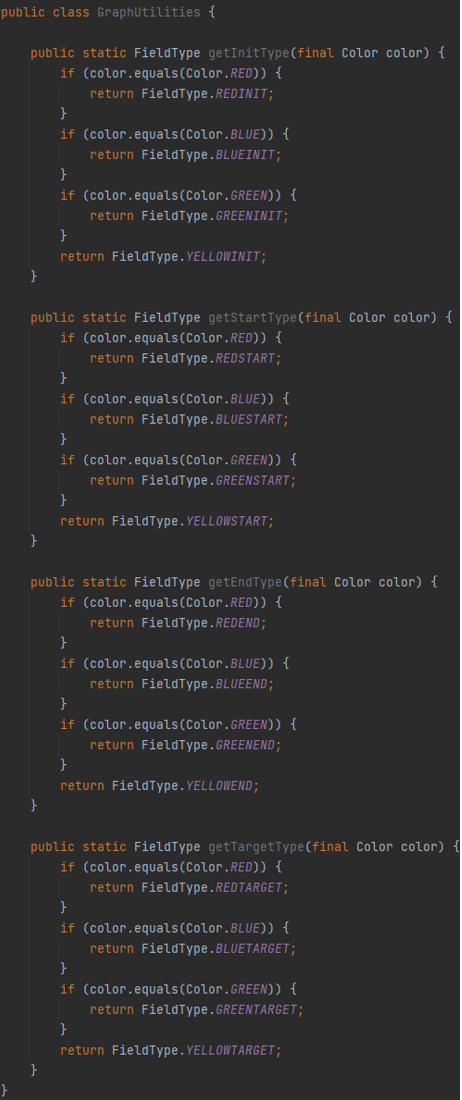
\includegraphics[scale=.55]{graphutilities}}
\caption{Switch-Statements [Eigene Darstellung aus \emph{IntelliJ}]}
\label{fig:graphutilities}
\end{figure}

\noindent Der Code-Smell bezieht sich auf die vier Methoden der \enquote{GraphUtilities}-Klasse (\hyperref[fig:graphutilities]{siehe Abbildung 7.3}). Der Switch-Statements Code Smell gilt auch hier, da die if-else-Statements einfach durch switch-Statements ersetzt werden können. Da sich diese Methoden alle um das \enquote{FieldType}-Enum drehen, wäre an dieser Stelle eine Implementierung der Methoden im Enum sinnvoller und würden den Code-Smell entfernen. 

\newpage
\noindent Das Enum wurde um fünf Instanzvariablen erweitert:

\begin{figure}[htbp]
\centering
\centerline{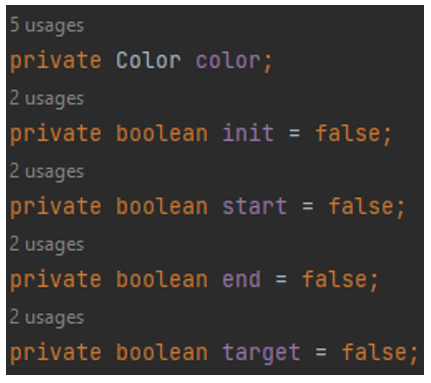
\includegraphics[scale=.55]{instanzvariablen}}
\caption{Erweiterung um fünf Instanzvariablen [Eigene Darstellung aus \emph{IntelliJ}]}
\label{fig:instanzvariablen}
\end{figure}

\noindent Außerdem wurden die vier Funktionalitäten aus den Graph-Utilities hinzugefügt, wie auf der nächsten Seite zu sehen ist.

\begin{figure}[htbp]
\centering
\centerline{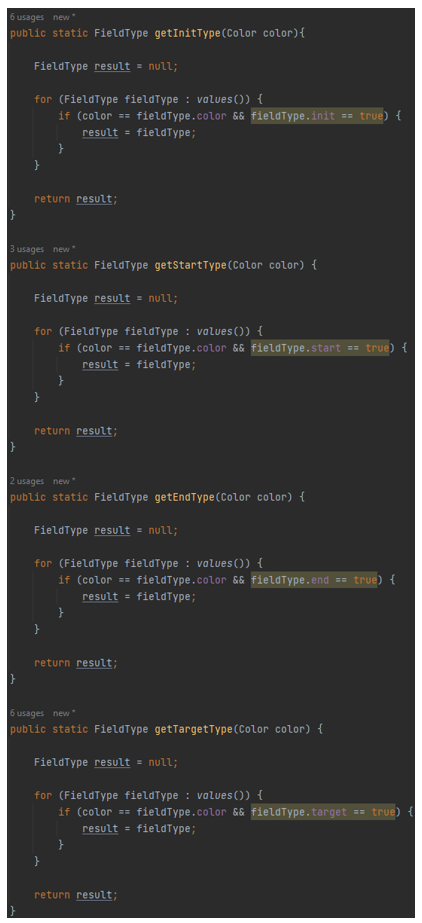
\includegraphics[scale=.8]{functionalities}}
\caption{Hinzufügen der vier Funktionalitäten [Eigene Darstellung aus \emph{IntelliJ}]}
\label{fig:funtionalities}
\end{figure}

\newpage
\section{2 Refactorings (6P)}
\emph{[2 unterschiedliche Refactorings aus der Vorlesung anwenden, begründen, sowie UML vorher/nachher
liefern; jeweils auf die Commits verweisen]}

\subsubsection{Extract Method}
\noindent Die Methode \enquote{saveGame} in der Klasse \enquote{GameIO} hat zuerst einen JSON-String erstellt und dann diesen mit dem aktuellen Zeitpunkt im Dateinamen abgespeichert. Beim Refactoring wurde hier einmal das Erstellen des JSON-Strings und das Generieren des aktuellen Zeitpunkts ausgelagert. Jetzt befindet sich nur noch der tatsächliche Abspeicherungsprozess in der Methode.

\begin{figure}[htbp]
\centering
\centerline{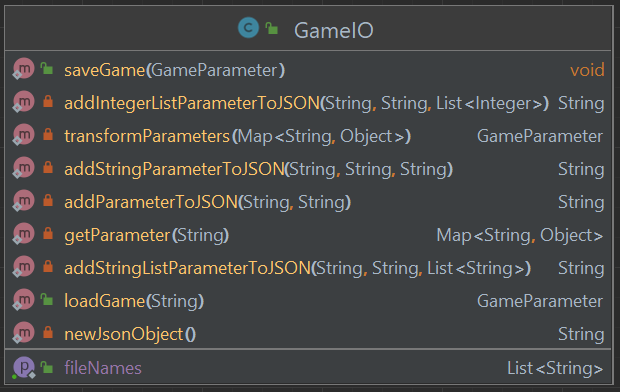
\includegraphics[scale=.5]{gameio1}}
\caption{Extract Method (vorher) [Eigene Darstellung aus \emph{IntelliJ}]}
\label{fig:gameio1}
\end{figure}

\newpage
\titlespacing*{\chapter}{0pt}{-30mm}{10pt}
\titleformat{\chapter}[display]
  {\normalfont\bfseries}{}{10pt}{\Huge\thechapter.\quad}
  
\chapter{Entwurfsmuster (8P)}
\pagestyle{scrheadings}
\clearscrheadfoot
\pagenumbering{arabic}
\setcounter{page}{35}
\ofoot[\pagemark]{\pagemark}
%\ohead[\headmark]{\headmark}
\onehalfspacing

\emph{[2 unterschiedliche Entwurfsmuster aus der Vorlesung (oder nach Absprache auch andere) jeweils
sinnvoll einsetzen, begründen und UML-Diagramm]}

\subsubsection{Entwurfsmuster: [Name] (4P)}
\subsubsection{Entwurfsmuster: [Name] (4P)}

\newpage
\titlespacing*{\chapter}{0pt}{-30mm}{10pt}
\titleformat{\chapter}[display]
  {\normalfont\bfseries}{}{10pt}{\Huge\thechapter.\quad}
  
\chapter{Anhang: Bedienungsanleitung}
\pagestyle{scrheadings}
\clearscrheadfoot
\pagenumbering{arabic}
\setcounter{page}{36}
\ofoot[\pagemark]{\pagemark}
%\ohead[\headmark]{\headmark}
\onehalfspacing

\noindent Zu Beginn eines Spiels wird zunächst die Anzahl an Spielern angegeben. Hierbei kann zwischen 2, 3 oder 4 ausgewählt werden.

\begin{figure}[htbp]
\centering
\centerline{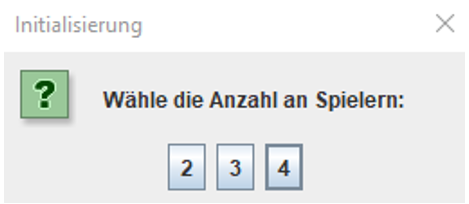
\includegraphics[scale=.5]{anleitung1}}
\caption{Auswahl der Spieleranzahl}
\label{fig:anleitung1}
\end{figure}

\noindent Nachdem die Spieleranzahl ausgewählt wurde, wird als nächstes die Anzahl der durch den Algorithmus gespielten Spielern ausgewählt. Es können bis zu 3 Spieler als Algorithmus initialisiert werden.

\begin{figure}[htbp]
\centering
\centerline{
\includegraphics[scale=.5]{anleitung2}}
\caption{Auswahl der Anzahl an simulierten Spielern}
\label{fig:anleitung2}
\end{figure}

\noindent Im nächsten Schritt werden die nicht-algorithmischen Spieler festgelegt. Hierbei können Spielern deren Namen zugewiesen werden. Alternativ können auch bereits existierende Spieler ausgewählt werden. Im Folgenden wurde Spieler 1 als neuer Spieler unter dem Namen Nadine angelegt. Als Spieler 2 wurde ein bereits existierender Spieler ausgewählt.

\newpage

% \begin{figure}[htbp]
% \centering
% \centerline{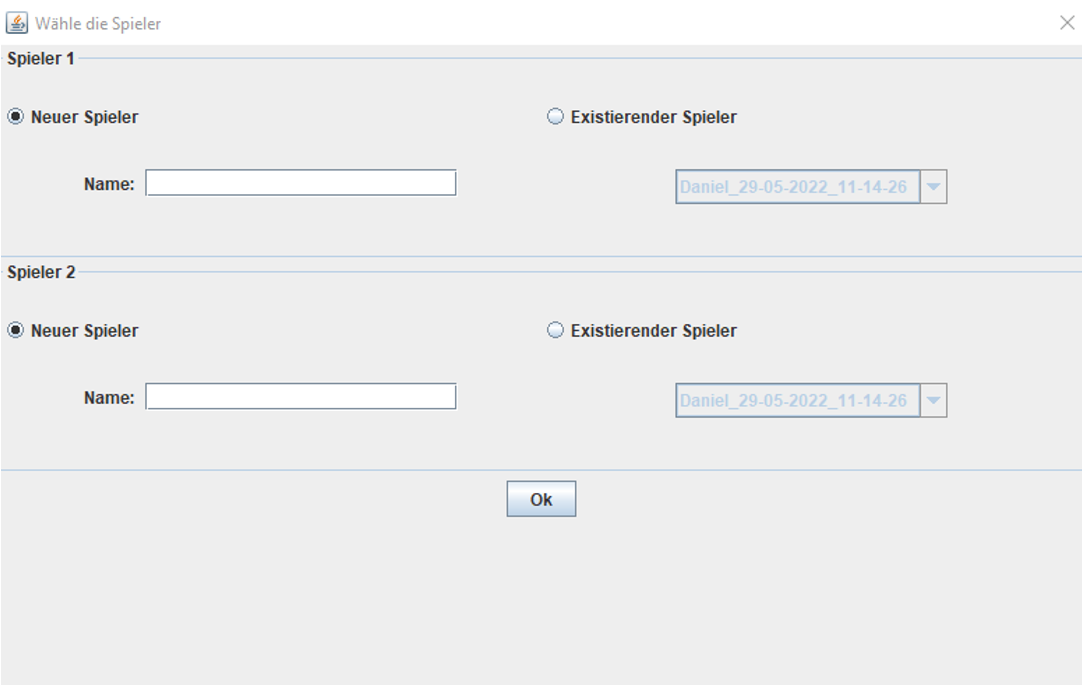
\includegraphics[scale=.6]{anleitung3}}
% \caption{Benennung der Spieler}
% \label{fig:anleitung3}
% \end{figure}

\begin{figure}[htbp]
\centering
\centerline{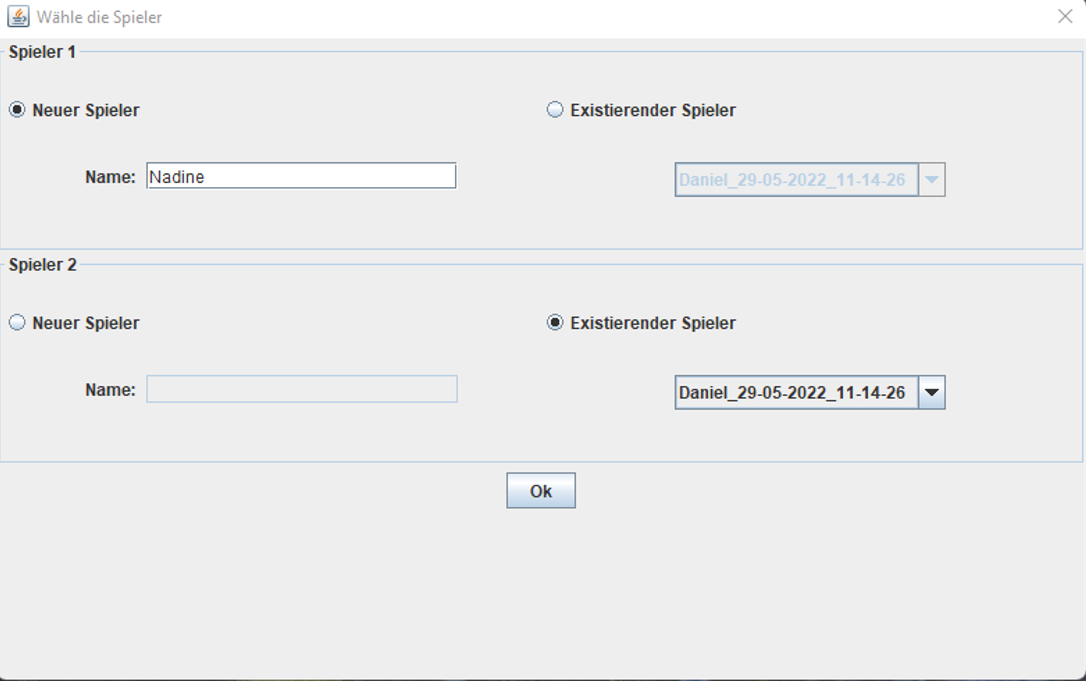
\includegraphics[scale=.6]{anleitung4}}
\caption{Benennung eines Spielers und Auswahl eines existierenden Spielers}
\label{fig:anleitung4}
\end{figure}

\noindent Nachdem Abschließend OK ausgewählt wurde beginnt das Spiel. Jeder Spieler erhält 4 Spielfiguren einer Farbe. Alle 4 Figuren stehen zu Beginn eines Spiels auf dem Feld A seiner Farbe. Die jeweiligen Spieler werden unterhalb des Spielfeldes mit Namen und ihrer jeweiligen Farbe angezeigt.

Die weißen Felder des Spielbretts stellen die Laufbahn C dar, die alle Spielfiguren zurücklegen müssen. Auf den jeweils farbigen Feldern auf der Laufbahn C beginnen die Spielfiguren ihren Weg über die weißen Felder. Auf der A-Feldern warten die Spielfiguren auf ihren Einsatz. Wer seine 4 Spielfiguren als erster in sein jeweiliges Ziel (Punkt D) gebracht hat, gewinnt das Spiel.

\newpage

\noindent Der Spieler, der an der Reihe ist, würfelt durch Klicken auf das Symbol \enquote{Fragezeichen in der Box} bei Punkt B. Wer keine Spielfigur auf der Laufbahn hat, weil alle Figuren geschlagen wurden oder zu Beginn des Spiels, darf dreimal würfeln. Die Spielfiguren, die auf den A-Feldern stehen, können nur mit einer \enquote{6} in das Spiel gebracht werden. Wird eine \enquote{6} gewürfelt, kann der Spieler selbst entscheiden mit welcher Figur er vom Startfeld A gehen möchte. Durch das Anklicken einer Figur wird diese ausgewählt und die Startposition auf der Laufbahn wird in Orange angezeigt. Wer eine \enquote{6} würfelt, hat nach seinem Zug einen weiteren Wurf frei. Erzielt er dabei wieder eine \enquote{6}, darf er nach dem Ziehen erneut würfeln. Bei einer \enquote{6} muss man eine neue Figur ins Spiel bringen, solange noch Spielfiguren auf dem eigenen A-Feldern stehen. Die neue Figur wird dann auf die Startposition der Laufbahn gestellt. Ist dieses Feld noch von einer anderen eigenen Spielfigur besetzt, muss diese Figur erst mit der \enquote{6} weitergezogen werden. Steht dagegen eine fremde Figur auf dem Feld, wird sie geschlagen. Wer eine \enquote{6} würfelt und keine Spielfigur mehr auf den B-Feldern hat, darf mit einer seiner Figuren auf der Laufbahn sechs Felder weiterziehen und dann noch einmal würfeln.

Eigene und fremde Figuren können übersprungen werden. Die besetzten Felder werden aber mitgezählt. Wer mehrere Spielfiguren auf der Laufbahn hat, kann sich aussuchen, mit welcher Figur er weiterzieht. Wer mit dem letzten Punkt seiner Augenzahl auf ein Feld tritt, das von einer fremden Spielfigur besetzt ist, schlägt diese Figur, welche wiederum automatisch zurück in den Startplatz gesetzt wird. 

\begin{figure}[htbp]
\centering
\centerline{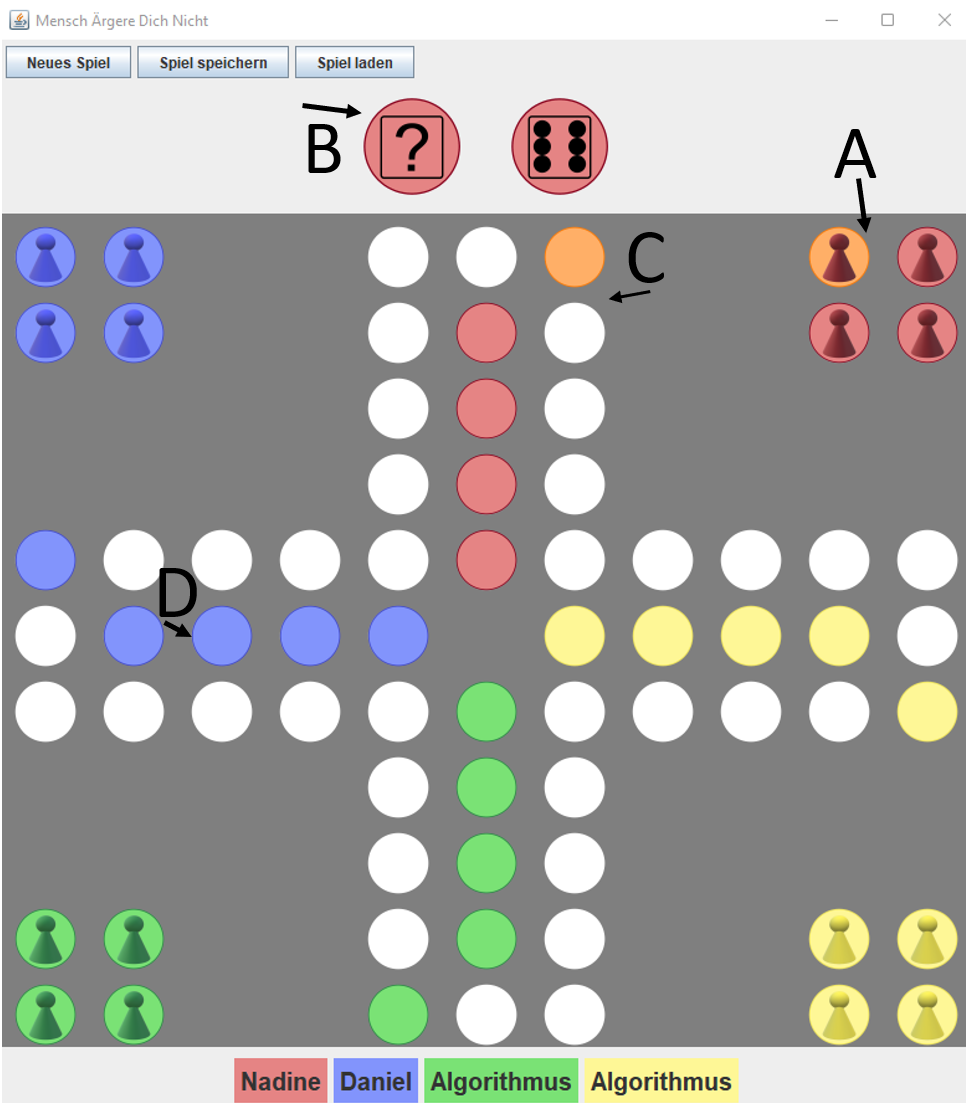
\includegraphics[scale=.6]{anleitung5}}
\caption{Hauptfenster der Anwendung mit Spielbrett}
\label{fig:anleitung5}
\end{figure}

% \newpage
% \titlespacing*{\chapter}{0pt}{-30mm}{10pt}
% \titleformat{\chapter}[display]
%   {\normalfont\bfseries}{}{10pt}{\Huge\thechapter.\quad}
  
% \chapter{Fragen an M. Müller}
% \pagestyle{scrheadings}
% \clearscrheadfoot
% \pagenumbering{arabic}
% \setcounter{page}{9}
% \ofoot[\pagemark]{\pagemark}
% %\ohead[\headmark]{\headmark}
% \onehalfspacing

% Fragen: 

% \begin{itemize}
%     %\item Dürfen wir \enquote{wir} in diesem Dokument verwenden?
%     %\item Wie genau soll die eigene Erklärung der Clean Architecture sein?
%     \item Siehe Kapitel SOLID / SRP: Ist es ok, dass wir die Klasse ControlMechanismFour nach refactoring nicht mehr haben?
%     \item Kapitel 3.2 OCP: Formulierung \enquote{Problem}
%     \item Kapitel 4.1 GRASP: Meint er mit negativ Beispiel einer geringen Kopplung eine starke Kopplung? 
%     \item Und soll die Kopplung in beiden fällen komplett aufgelöst werden oder nur zu einer geringen Kopplung gemacht werden?
%     \item Verstehen wir das richtig, dass man im DDD nur ein Repository haben kann, wenn man einen persistenten Speicher hat?
% \end{itemize}